\documentclass[serif]{beamer}

% Information to be included in the title page:

\title{Deep Hedging}

\author{Bent Müller}
\institute{University of Hamburg, Department of Mathematics}
\date{12.6.2023}

% Standard beamer class setup, configure as needed

\usepackage{tikz}
\usetikzlibrary{automata, positioning}

\setbeamertemplate{headline}[default]
\setbeamertemplate{caption}[numbered]
\setbeamertemplate{navigation symbols}{}
\mode<beamer>{\setbeamertemplate{blocks}[rounded][shadow=true]}
\setbeamercovered{transparent}
\setbeamercolor{block body example}{fg=blue, bg=black!20}

\useoutertheme[subsection=true]{miniframes}
\usetheme{Frankfurt}

% Definition of new commands
\def\R{{\mathbb R}}
\def\P{{\mathbb P}}
\def\E{{\mathbb E}}
\def\N{{\mathbb N}}
\def\O{{\Omega}}

\def\cF{{\mathcal F}}

\def\cP{{\mathcal P}}
\def\cG{{\mathcal G}}
\def\cX{{\mathcal X}}
\def\cY{{\mathcal Y}}

\def\BM{{\text{BM}}}
\def\RN{{\text{RN}}}
\def\Var{{\text{Var}}}
\def\Cov{{\text{Cov}}}
\def\riskNeutralQ{{\mathbb Q}}
\def\F{{\mathbb F}}

\def\vs{{\vspace{0.5cm}}}

% These are specifically for deep hedging
\def\Hu{{\mathcal H^u}}
\def\H{{\mathcal H}}
\def\L{{\mathcal L}}

% New additions for complete market model
\def\ps{{(\O, \cF, \P)}}
\def\fm{{(\O, \cF, \P, \F, S)}}

\begin{document}

\begin{frame}
    \titlepage
    \footnote{
        Original Paper: \cite[Deep Hedging]{bühler2018deep}
    }
\end{frame}

% TOC I sent to supervisor
% 1. The general problem of hedging a portfolio of derivatives (recap)
% 2. Setup in the paper
% 2.1 Different (convex) risk measures
% 2.2 From risk measures to hedging strategies
% 3. Neural Networks Introduction
% 3.1 Universal Approximation Theorem
% 3.2 Learning Optimal Hedging Strategies
% 3.3 Neural Network Architectures (recurrent and simple feed forward)
% 4. Numerical Results from the Paper
% 4.1 Hedging in the Heston Model
% 4.2 Hedging in a Multi-Asset Market (underlying + variance swap)
% 4.3 Choosing risk measures to optimize for

\section{Table of Contents}
\begin{frame}
    \tableofcontents
\end{frame}

\section{Hedging a Portfolio of Derivatives}

\subsection{Recap from the Lecture}
\begin{frame}
    \frametitle{Notation}
    \begin{itemize}
        \only<1>{
        \item $\O := \{ \omega_1, \omega_2, \dots, \omega_N \}$ is our \textbf{discrete} set of outcomes.
        \item $\cF := 2^\O$ the $\sigma$-algebra of all subsets of $\O$, so that is
              $\fm$ our financial market.
              }
              \only<1-2>{
        \item $\cX := \{X: \O \to \R\}$ is the set of all real-valued random variables.
        \item $\rho: \cX \to \R$ is a risk measure.
              }
              \only<2-3>{
        \item $l: \R \to \R$ \textbf{continuous, convex and non-decreasing} is called a loss function.
        \item $\rho_l: \cX \to \R$, where $\rho_l (X) := \inf_{w \in \R} \{ w + \E [ l (-X -w) ] \}$ defines
              a convex risk measure, a so-called \textbf{Optimized Certainty Equivalent} (OCE) risk measure
              (Lemma 3.16).
        \item $S^i_t : \O \to \R_{\geq 0}$
              is the $\cF_t$-measurable price of the $i$-th risky asset
              at time $t$
              for $0 \leq t \leq T$ and $0 \leq i \leq d$.
              }
        \item $\Hu := \{ \phi : \O \to \R^{d+1} \; | \; \forall 0 \leq t \leq T:
                  \phi_{t+1} \text{ is } \cF_t \text{-measurable and } \phi_{-1} = \phi_T = 0 \} $ is the set of
              unconstrained hedging strategies.
    \end{itemize}
\end{frame}

\subsection{Hedging under Transaction Costs and Market Frictions}

\begin{frame}[t]
    \frametitle{Trading with Transaction Costs}
    For $\delta$ a trading strategy, we define
    $$C_T (\delta) := \sum_{t=0}^T c_t (\delta_t - \delta_{t-1})$$
    as the \textbf{cumulative transaction cost} of
    trading using $\delta$ up to time $T$.
    $c_t : \R^{d+1} \to \R^+$ is a non-negative \textbf{adapted cost process}
    satisfying $\forall t: c_t (0) = 0$.
    \vs

    This makes different transaction costs possible, like:
    \begin{itemize}
        \only<1>{
        \item Proportional Transaction Costs:
              $$c_t (n) = \sum_{i=0}^d c_t^i S_t^i | n^i |$$
              for a transaction $n \in \R^{d+1}$.
              }
              \only<2>{
        \item Fixed Transaction Costs:
              $$c_t (n) = \sum_{i=0}^d c_t^i 1_{|n^i| > 0}$$
              for a transaction $n \in \R^{d+1}$.
              }
              \only<3>{
        \item Or even volatility dependent transaction costs which we won't consider here.
              In this case $c_t$ might increase with high volatility.
              }
              \only<4>{
        \item If the agent is allowed to trade in other options to hedge $-Z$,
              there might be additional costs for high volatility.
              This is called the \textbf{cost of volatility} and can be modeled
              if we allow $c_t$ to depend on the Black \& Scholes \textbf{Vega}
              of each traded asset.
              }
    \end{itemize}
\end{frame}

\begin{frame}
    \frametitle{Fundamental Problem}
    A hedging agent then wishes to achieve
    the optimal hedge for a given liability $-Z$.
    \[
        \pi (-Z) := \inf_{\delta \in \H} \rho (
        -Z + (\delta \cdot S)_T - C_T (\delta)
        )
    \]
    $\pi (-Z)$ is the risk of the \textbf{optimal hedge} possible when hedging
    using strategies in $\H$.
    Then
    $$p(Z) = \pi (-Z) - \pi (0)$$
    is the \textbf{indifference price} at which the agent would be
    indifferent between holding $-Z$ and not holding any position.
\end{frame}

\begin{frame}
    \frametitle{Fundamental Problem}
    At time $T$, the agent's wealth is then given by
    $$p_0 - Z + (\delta \cdot S)_T - C_T (\delta)$$
    where $p_0$ is the amount she received for selling $Z$ in the first place. \\
    \vs
    Note that $p_0$ may also be given externally and must not be the
    indifference price $p(Z)$.
\end{frame}

\subsection{Conditional Value at Risk}

\begin{frame}
    \frametitle{Conditional Value at Risk}
    For any $X \in \L^1 (\O, \cF, \P)$ and $\alpha \in (0,1)$,
    the \textbf{Conditional Value at Risk}
    is defined as
    $$\text{CVaR}_\alpha (X) := \frac{1}{\alpha} \int_0^\alpha VaR_u (X) du$$
    where $VaR_\lambda (X)$ is the \textbf{Value at Risk} at level $\lambda$ defined as
    $$VaR_\lambda (X) := \inf \{ x \in \R \; | \; \P (X \leq x) \geq \lambda \}.$$
\end{frame}

\begin{frame}
    \frametitle{Conditional Value at Risk of S\&P 500 Daily Returns}
    \begin{figure}
        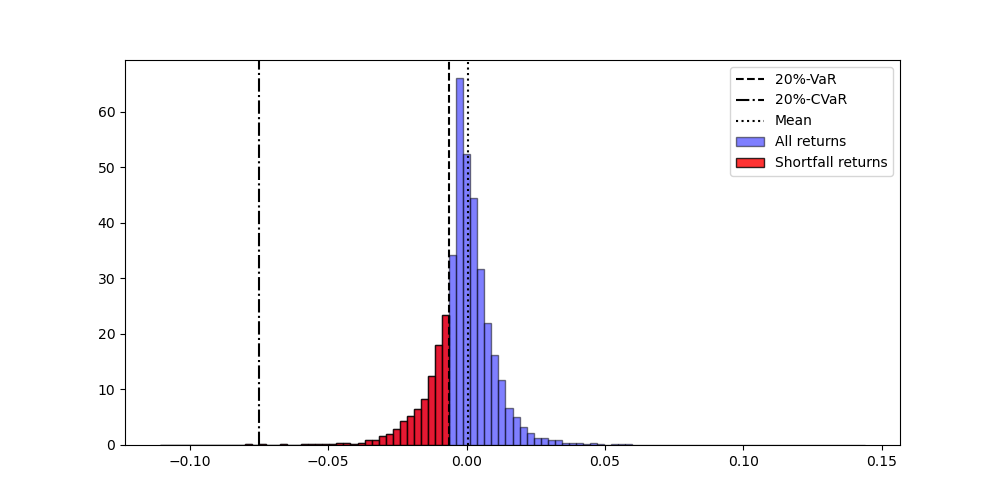
\includegraphics[width=1.0\textwidth]{./images/cvar_sp500_example.png}
        \caption{Conditional Value at Risk of S\&P 500 Daily Returns since 1993-02-01}
    \end{figure}
\end{frame}

\section{Introduction to Neural Networks}

\begin{frame}
    \frametitle{Single Layer Perceptron}
    For integers
    $d_{in}, d_{out} \in \N$ and
    an activation function \footnotemark
    \footnotetext{
        nonlinear, continuous and differentiable a.e.
    }
    $\sigma: \R \to O$,
    we define a \textbf{single layer perceptron} as
    the following function
    \[
        \text{F}_{W, b}: \R^{d_{in}} \to \R^{d_{out}}, \;
        x \mapsto \sigma (W x + b).
    \]
    \only<1>{
        Note that
        \begin{itemize}
            \item $O \subseteq \R$ is the image of $\sigma$,
            \item $W \in \R^{d_{out} \times d_{in}}$ is called the \textbf{weight matrix},
            \item $b \in \R^{d_{out}}$ is called the \textbf{bias vector} and
            \item $\sigma$ is applied component-wise.
        \end{itemize}
    }
    \only<2>{
        \\ \vs
        We shorten the parameters of the network to $\theta := (W, b)$
        and will simply write $\text{F}_\theta$.
    }
\end{frame}

\begin{frame}
    \frametitle{Common Activation Functions}
    \begin{figure}
        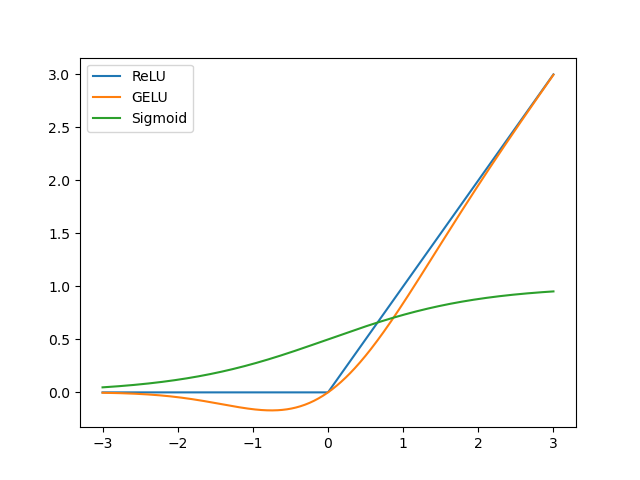
\includegraphics[width=0.8\textwidth]{./images/activation_functions.png}
        \caption{Common Activation Functions}
    \end{figure}
\end{frame}

\begin{frame}
    \frametitle{Feed Forward Networks}
    For $L, d_1, \ldots, d_L \in \N$
    and activation function $\sigma$,
    we define a \textbf{feed forward network} (FFN) as
    \[
        \text{FFN}: \R^{d_1} \to \R^{d_L}, \;
        x \mapsto \text{F}_{\theta_L}^{(L)} \circ \ldots \circ \text{F}_{\theta_1}^{(1)} (x).
    \]
    We call
    \begin{itemize}
        \item $L$ the depth, or the number of layers, of the network,
        \item $d_1$ the input dimension,
        \item $d_L$ the output dimension,
        \item $d_2, \ldots, d_{L-1}$ the hidden dimensions and
        \item $F_{\theta_l}^{(l)}: \R^{d_l} \to \R^{d_{l+1}}$ the $l$-th layer of the network.
    \end{itemize}
\end{frame}

\subsection{Universal Approximation Theorem}

\section{Deep Hedging}

\subsection{Why Use Neural Networks?}
\subsection{Deep Hedging as Presented in The Paper}
\subsection{Pricing using Deep Hedging}

% And make the references slide using bibtex
\section{References}
\begin{frame}
    \frametitle{References}
    \bibliographystyle{apalike}
    \bibliography{references}
\end{frame}

\end{document}
